\chapter{Funzione di Eulero e RSA}

\section{Funzione di Eulero}

Si dice \textbf{funzione di eulero} (o \textbf{toziente di eulero}) l'applicazione \fcolorbox{red}{white}{$\phi: \mathbb{N} \mapsto \mathbb{N}$} che associa ad ogni $n \in \mathbb{N}$ il numero di interi compresi fra 1 e $n$ coprimi con $n$. Se $n$ è \textbf{primo} allora si può dire che $\phi(n) = n - 1 \; \forall n$ primo. \newline
\textbf{Proprietà}:
\begin{itemize}[nosep]
    \item Il numero di elementi invertibili in $\mathbb{Z}_n \; (\forall n \geq 2)$ è esattamente $\phi(n)$.
    \begin{boxA}
        \textcolor{olive}{\textbf{Dimostrazione}}: fissato $n \geq 2$, un elemento $x \in \mathbb{Z}$ è invertibile \textbf{se e solo se} $\exists y \in \mathbb{Z} \; \text{t.c.} \; x \cdot y \equiv_n 1$ questa è una congruenza lineare che ammette soluzioni \textbf{se e solo se} $\gcd (x, y) = 1$ ovvero se $x$ e $y$ sono \textbf{coprimi}. Quindi il numero di elementi invertibili in $\mathbb{Z}_n$ è pari al numero di elementi coprimi ad $n$ in $\mathbb{Z}_n$ che è la stessa definizione di $\phi(n)$
    \end{boxA}
    \item $\forall n \in \mathbb{N}$, il numero di stelle (distinte) a $n$ punte è:

    {\centering
        $\frac{\phi(n) - 2}{2}$
    \par}

    \item se $p \in \mathbb{Z}^+$ è un numero primo allora $\phi(p) = p - 1$.
    \item se $p \in \mathbb{Z}^+$ è un numero primo allora $\phi(p^h) = p^h - p^{h - 1}, \; \forall h \geq 1$
    \item se $p, q \in \mathbb{Z}^+$ sono due numeri primi distinti allora $\phi(pq) = \phi(p) \cdot \phi(q)$
\end{itemize}
\begin{flushleft}
    \textcolor{blue}{\textbf{Corollario}}: se $n = p_1^{h_1} \cdot p_2^{h_2} \cdot ... \cdot p_r^{h_r}$, con $p_i$ \textbf{primi distinti} ($i \in \mathbb{N}_r)$ allora:

    {\centering
        $\phi(n) = \phi(p_1^{h_1}) \cdot \phi(p_2^{h_2}) \cdot ... \cdot \phi(p_r^{h_r})$
    \par}
    ovvero posso calcolare il \textbf{toziente di eulero} per ogni $n \in \mathbb{Z}$ se conosco la sua \textbf{fattorizzazione}.
\end{flushleft}

\newpage
\begin{flushleft}
    \textbf{Teorema di Eulero-Fermat} \\
    $\forall n \in \mathbb{N}$ e $\forall a \in \mathbb{Z}$ tale che $\gcd (a, n) = 1$, si ha:
    
    {\centering
        $a^{\phi(n)} \equiv_n 1$
    \par}

    \begin{boxA}
        \textcolor{olive}{\textbf{Dimostrazione}}: dimostriamo il teorema per \textbf{induzione} con $n = p^h$ con p \textbf{primo} e $h_i \in \mathbb{N}, \; \forall i \in \mathbb{N}$

        \textcolor{red}{\textbf{Passo Iniziale}} \newline
        se $h = 1$, significa che $n = p^1 = p$ primo quindi la tesi non è altro che il \textbf{piccolo teorema di fermat}.

        \textcolor{red}{\textbf{Passo Induttivo}}
        
        {\centering
            \begin{minipage}[t]{0.45\textwidth}
                \textbf{Hp.} $\forall a \in \mathbb{Z} \; | \; \gcd (a, p^h) = 1$ \\
                $\Longrightarrow \;\; a^{\phi(p^h)} \equiv 1 \; \text{mod} \; p^h$
            \end{minipage}
            \hfill
            \begin{minipage}[t]{0.45\textwidth}
                \textbf{Th.} $\forall a \in \mathbb{Z} \; | \; \gcd (a, p^{h + 1}) = 1$ \\
                $\Longrightarrow \;\; a^{\phi(p^{h + 1})} \equiv 1 \; \text{mod} \; p^{h + 1}$
            \end{minipage}
        \par}
        Per la \textbf{proprietà} del \textit{toziente di eulero} $\phi(p^h) = p^h - p^{h - 1}$
        \begin{align*}
            \phi(p^{h + 1}) &= p^{h + 1} - p^h \\
            &= p \cdot (p^h - p^{h - 1}) \\
            &= p \cdot \phi(p^h)
        \end{align*}
        Quindi $a^{\phi(p + 1)} = a^{p \cdot \phi(p^h)}$ che si può rapprensentare anche come \fcolorbox{red}{white}{$(a^{\phi(p^h)})^p$}. Per \textbf{Hp.} induttiva $a^{\phi(p^h)} \equiv 1 \; \text{mod} \; p^h$, ovvero $\exists k \in \mathbb{Z} \; | \; a^{\phi(p^h)} = 1 + k \cdot p^h$ andando a sostituire otteniamo:

        {\centering
            $(a^{\phi(p^h)})^p = (1 + k \cdot p^h)^p$
        \par}
        che corrisponde alla \textbf{potenza di un binomio} (calcolabile con il \textbf{Binomio di Newton} $\rightarrow (A + B)^n = \underset{r=0}{\overset{n}{\sum}} \binom{n}{r} A^{n - r} \cdot B^r$), quindi avremo:

        {\centering
            $(1 + k \cdot p^h)^p = 1 + \binom{p}{1}(k \cdot p^h)^1 + \binom{p}{2}(k \cdot p^h)^2 + ... + \binom{p}{p}(k \cdot p^h)^p$
        \par}
        Ad eccezione del ``$1 +$'' tutti gli altri membri sono multipli di $p^{h + 1}$, infatti: \\
        $\binom{p}{1} (k \cdot p^h)^1 = p \cdot kp^h = k \cdot \fcolorbox{red}{white}{$p^{h + 1}$}$ \\
        $\binom{p}{1} (k \cdot p^h)^2 = \frac{p(p - 1)}{2} \cdot k^2 \cdot p^{2h} = \frac{p - 1}{2} \cdot k^2 \cdot \fcolorbox{red}{white}{$p^{2h + 1}$}$ \\
        $\vdots$ \\
        $\binom{p}{p} (k \cdot p^h)^p$ \\
        Quindi tutti i fattori sono multipli di $p^{h + 1}$ quindi $\text{mod} p^{h + 1}$ si annullano quindi avremo che:
        
        {\centering
            \fcolorbox{red}{white}{$(1 + k \cdot p^h)^p \equiv 1 \; \text{mod} \; p^{h + 1}$}
        \par}
        Questo dimostra il passo induttivo e quindi la nostra \textbf{Th.}
    \end{boxA}
    \begin{boxA}
        \textcolor{olive}{\textbf{Dimostrazione}}: ora dimostriamo il teorema (\textbf{caso generale}) con $n = p_1^{h_1} \cdot p_2^{h_2} \cdot ... \cdot p_r^{h_r}$ con $p_i$ \textbf{primi distinti} e $h_i \in \mathbb{N}, \; \forall i \in \mathbb{N}_r$. Voglio provare che $\forall a \in \mathbb{Z} \; | \; \gcd (a, n) = 1$ e che quindi $a^{\phi(n)} \equiv_n 1$ (è la nostra \textbf{Th.})
        \begin{itemize}[nosep]
            \item so che $a^{\phi(p_i^{h_i})} \equiv 1 \; \text{mod} \; p_i^{h_i} \; \forall i \in \mathbb{N}_r$ dato che $\gcd (a, p_i^{h_i}) = 1$, perché se $a$ è \textbf{coprimo} con $n$, allora è \textbf{coprimo} anche con i singoli fattori.
            \item d'altra parte so che $\phi(n) = \phi(p_1^{h_1}) \cdot \phi(p_2^{h_2}) \cdot ... \cdot \phi(p_r^{h_r})$, quindi $\phi(p_i^{h_i})|\phi(n) \; \forall i \in \mathbb{N}_r$, cioè 
            
            {\centering
                \fcolorbox{red}{white}{$\frac{\phi(n)}{\phi(p_i^{h_i})} \in \mathbb{Z}$}
            \par}
            \item elevando entrambi i membri della prima equivalenza a tale esponente ottendo:
            \begin{align*}
                a^{\phi(p_i^{h_i})} &\equiv 1 \; \text{mod} \; p_i^{h_i} \\
                (a^{\phi(p_i^{h_i})})^{\frac{\phi(n)}{\phi(p_i^{h_i})}} &\equiv (1)^{\frac{\phi(n)}{\phi(p_i^{h_i})}} \; \text{mod} \; p_i^{h_i} \\
                (a^{\cancel{\phi(p_i^{h_i})}})^{\frac{\phi(n)}{\cancel{\phi(p_i^{h_i})}}} &\equiv (1)^{\frac{\phi(n)}{\phi(p_i^{h_i})}} \; \text{mod} \; p_i^{h_i} \\
                a^{\phi(n)} &\equiv 1 \; \text{mod} \; p_i^{h_i} \; \forall i \in \mathbb{N}_r
            \end{align*}
            Ciò significa che $a^{\phi(n)} - 1$ è multiplo di $p_i^{h_i} \; \forall i \in \mathbb{N}_r$, ma poiché i $p_i$ sono \textbf{primi distinti}, si ha $a^{\phi(n)} - 1$ multiplo di $p_1^{h_1} \cdot p_2^{h_2} \cdot ... \cdot p_r^{h_r} = n$ e quindi avremo che:

            {\centering
                \fcolorbox{red}{white}{$a^{\phi(n)} \equiv_n 1$}
            \par}
        \end{itemize}
    \end{boxA}

    \textbf{Formulazione equivalente del Teorema di Eulero-Fermat} \\
    $\forall n \in \mathbb{N}$ e $\forall a \in \mathbb{Z}$ tale che $\gcd (a, n) = 1$, si ha:
    
    {\centering
        $a^{\phi(n) + 1} \equiv a \; \text{mod} \; n$
    \par}
    Inoltre $a^{h \cdot \phi(n) + 1} \equiv a \; \text{mod} \; n$ \\
    \textcolor{red}{\textbf{N.B.}}: se $n$ non è primo, in generale l'ipotesi $\gcd (a, n) = 1$ \textbf{non} può essere rimossa.

    $\Longrightarrow$ \textcolor{blue}{\textbf{intero libero da quadrati}}: un intero $n \in \mathbb{N}$ si dice \textbf{libero da quadrati} se la sua scomposizione è il prodotto di primi disgiunti: \fcolorbox{red}{white}{$n = p_1 \cdot p_2 \cdot ... \cdot p_r$}
\end{flushleft}

\newpage
\begin{flushleft}
    \textbf{Teorema di Eulero-Fermat Generalizzato}: se $n \in \mathbb{Z}$ è un \textit{intero libero da quadrati}, allora:

    {\centering
        $a^{\phi(n) + 1} \equiv a \; \text{mod} \; n \quad \forall a \in \mathbb{Z}$
    \par}
    Inoltre $a^{h \cdot \phi(n) + 1} \equiv a \; \text{mod} \; n \quad \forall a \in \mathbb{Z}, \; \forall h \in \mathbb{Z}^+$

    \begin{boxA}
        \textcolor{olive}{\textbf{Dimostrazione}}: supponiamo $n = p_1 \cdot p_2 \cdot ... \cdot p_r$ con $p_i$ \textbf{primo} $\forall i \in \mathbb{N}_r$ e $p_i \neq p_j, \; \forall i \neq j$ e consideriamo il sistema di congruenze lineari: \\
        $\begin{cases}
            x \equiv a \; \text{mod} \; p_1 \\
            x \equiv a \; \text{mod} \; p_2 \\
            \vdots \\
            x \equiv a \; \text{mod} \; p_r
        \end{cases}$ \\
        Per il \textbf{Teorema Cinese del Resto} $\exists ! \text{Sol mod}(p_1 \cdot p_2 \cdot ... \cdot p_r)$ cioè $n$. Banalmente $\overline{x} = a$ è soluzione del sistema. Quindi per provare la \textbf{Th.} basta verificare che anche $a^{k \cdot \phi(n) + 1}$ è soluzione del sistema. Sappiamo che $\phi(n) = \phi(p_1 \cdot ... \cdot p_r) = \phi(p_1) \cdot ... \phi(p_r)$. Quindi $\forall i \in \mathbb{N}_r$ avremo che $\phi(n) = \phi(p_i) \cdot [\underset{j \neq i}{\prod}\phi(p_j)]$, che rappresenta la produttoria degli altri numeri primi escluso $p_i$ e la chiameremo $S_i \in \mathbb{Z}$. Allora:
        \begin{align*}
            a^{k \cdot \phi(n) + 1} &= a^{k \cdot S_i \cdot \phi(p_i) + i} & \forall i \in \mathbb{N}_r \\
            &= a^{k \cdot S_i \cdot (p_i - 1) + 1} & k \cdot S_i \in \mathbb{Z} \\
            &= a^{k \cdot S_i \cdot (p_i - 1) + 1} \equiv a \; \text{mod} \; p_i & \forall a \in \mathbb{Z}
        \end{align*}
        L'ultimo passaggio è possibile per il \textbf{corollario derivante dal piccolo teorema di fermat}. Quindi $a^{k \cdot \phi(n) + 1}$ verifica la $i$-esima congruenza del sistema, si può quindi dimostrare analogamente per le restanti $r - 1$ congruenze lineari del sistema.
    \end{boxA}
\end{flushleft}

\section{Codici Correttori e Rilevatori}

\begin{flushleft}
    \textbf{Alfabeto}: insieme finito $\mathbb{F}$, ad esempio nel caso dell'alfabeto binario avremo che $\mathbb{F} = \{0, 1\}$ \\
    \textbf{Parole}: Sequenze finite di elemnti di $\mathbb{F}$, ad esempio se consideriamo la parola binaria: $100100_{(2)}$ questa sarà una parola di lunghezza 6. \\
    \textbf{Codice} (\textbf{a blocchi}): Un qualunque sottoinsieme non vuoto $\mathbb{C} \subseteq \mathbb{F}^n$, ad esempio $\mathbb{C} = \{00000, 01011, 10101, 11110\}$ è un codice binario di lunghezza 5. \newline

    \textbf{N.B.} nell'addizione binaria, la somma di $m$ bit è 0 quando tra di essi vi è un numero pari di bit uguale 1.

    \textbf{Controllo di Parità}: il controllo di parità è un bit che, aggiunto ad una parola binaria, è: \textbf{0} se la parola conteneva un numero pari di bit a 1, \textbf{1}, se la parola conteneva un numero dispari di bit a 1.
\end{flushleft}

\subsection{Sistemi di Comunicazione}
Nei canali di comunicazione, sono presenti un codificatore (lato mittente) e un decodificatore (lato destinatario). Il compito del codificatore, conoscendo la regola di codificazione usata dal mittente, è di tentare di ricostruire, in caso di messaggio disturbato, la versione originale.
\begin{itemize}[nosep]
    \item \textbf{Decodificatore a controllo di parità}: Si limita a controllare se la somma dei bit fa 0 oppure no, in caso negativo, si limita a segnalare che nella trasmissione della parola, è avvenuto un errore. Questo codice rilevatore si chiama \textbf{codice 1-rilevatore}, perché si accore di un errore, ma non riesce a correggerlo, in quanto non riesce a stabilire quale bit è stato invertito.
    \item \textbf{Codice ripetitivo}: viene inviato lo stesso messaggio di lunghezza $k$ più volte (ad esempio triplo $n = 3k$)
    \begin{enumerate}[nosep]
        \item suddivide la parola ottenuta in parole parziali.
        \item partendo dal primo, si controlla l'$i$-esimo caratterre di ogni parola e, se una maggioranza dei caratteri coincide, allora si considera tale carattere come quello corretto.
        \item se non c'è una maggioranza, il processo emette una comunicazione di errore e si ferma. Altrimenti, si itera il procedimento per tutti i caratteri.
        \item infine, emette la parola ottenuta.
    \end{enumerate}
    \textbf{Problema}: se i caratteri errati compongono la maggioranza, allora il codice ripetitivo considera il bit errato come corretto, per ovviare a questo problema bisogna avere una probabilità di errore dei singoli bit bassa. \textbf{Tasso di informazione}: $\frac{1}{d}$, dove $d$ è il numero di ripetizioni del messaggio.
    \item \textbf{Codice binario di Hamming}: il codificatore aggiunge al blocco di $k$ bit, $k - 1$ bit di controllo secondo la seguente regola:
    
    \begin{figure}[h]
        \centering
        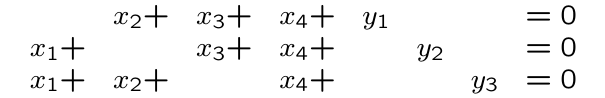
\includegraphics[width=0.45\textwidth]{img/hamming}
        \caption{Esempio con $k = 4$}
    \end{figure}
    Verrà poi inviata la sequenza $M = x_1x_2x_3x_4y_1y_2y_3$, il decodificatore calcolerà le 3 somme di controllo:
    \begin{itemize}[nosep]
        \item se sono tutte e tre uguali a 0, allora il decodificatore assume che non ci siano stati errori di comunicazione.
        \item se una somma è diversa da 0, allora il decodificatore assume che l'errore sia avvenuto sul bit di controllo.
        \item se 2 su 3 sono diverse da 0, allora il decodificatore assume che il bit scambiato è quello non presente nella terza somma.
        \item se sono tutti e tre diversi da 0, allora l'errore è nel quarto bit (presente in tutte le somme)
    \end{itemize}
    In questo caso avremo un \textbf{Tasso di informazione}: $\frac{k}{n} = \frac{k}{k +(k - 1)}$, solitamente migliore del codice ripetitivo.
    \item \textbf{Codice ISBM}:

    \begin{figure}[h]
        \centering
        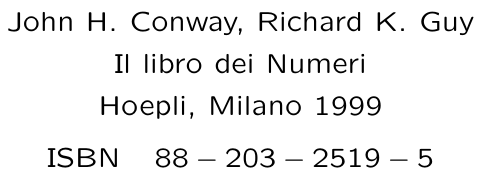
\includegraphics[width=0.35\textwidth]{img/isbm}
        \caption{International Standard Book Number}
    \end{figure}
    \begin{itemize}[nosep]
        \item 88: indica che il libro è stato pubblicato in Italia.
        \item 203: indica l'editore.
        \item 2519: identificativo di quel libro, dalla casa editrice.
        \item 5: cifra di controllo
    \end{itemize}
    Il numero complessivo è ammissibile come numero \textbf{ISBM} se la somma pesata $10 \cdot Y_10 + 9 \cdot Y_9 + ... + 1 \cdot Y_1$ da un risultato divisibile per 11. La cifra di controllo serve quindi per riconoscere errori di trasmissione, dovuti ad errori di scrittura o di comunicazione del numero ISBM.
\end{itemize}
\begin{flushleft}
    \textbf{Canale di Trasmissione}: Il canale binario simmetrico è uno dei modelli di trasmissione più utilizzati: accetta in ingresso e trasmette in usicta solo i caratteri $\mathbb{F} = \{0, 1\}$. \textbf{Probabilità cruda di errore} (\textbf{p}): è la probabilità con la quale, un bit entrato nel canale viene trasformato dal rumore nel bit complementare. Quindi, in una parola $x_1x_2...x_m$ avvengono $t$ errori con una probabilità pari:
    
    {\centering
        \fcolorbox{red}{white}{$(1 - p)^{m - t} \cdot p^t$}.
    \par}
\end{flushleft}

\newpage
\subsection{Interleaving}
\begin{flushleft}
    Si è supposto che i disturbi coinvolgano i caratteri in maniera indipendente, tuttavia, in realtà se un carattere viene alterato, allora è più facile che anche quelli vicini a lui vengano alterati. Il metodo di \textit{interleaving} è efficace control scrosci di errori (\textbf{burst errors}), che non siano troppo lunghi.

    \textcolor{orange}{\textbf{Esempi}} \\
    Data la sequenza da trasmettere: $10 \; 00 \; 01 \; 11 \; 11 \; 11 \; 01 \; 10 \; 00 \; 00 \; 10 \; 10 \; ...$
    Adottando il codice binario di lunghezza 5:$x_1x_2y_1y_2y_3$, dove $y_1 = x_1$, $y_2 = x_2$ e $y_3 = x_1 + x_2$, otteniamo delle parole che, memorizzate a gruppi di 4 creano delle matrici:

    \begin{figure}[h]
        \centering
        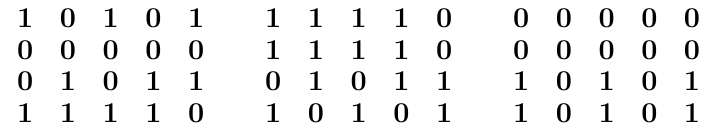
\includegraphics[width=0.45\textwidth]{img/interleaving_1}
    \end{figure}
    Il contenuto di tali matrici viene inviato colonna per colonna. Supponiamo che avvengano dei disturbi ai bit: 3, 5, 6, 39, 40, 41, 42, 59 e 60. Quindi il messaggio letto dal decodificatore sarà:

    \begin{figure}[h]
        \centering
        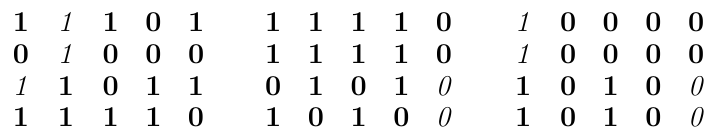
\includegraphics[width=0.45\textwidth]{img/interleaving_2}
    \end{figure}
    Riesce a decodificare correttamente i bit, perchè ogni riga ha al massimo 1 errore. I vantaggi dell'interleaving, tuttavia, si pagano con una maggiore complessità per la comunicazione e con dei ritardi nella trasmission dei dati.

    \textbf{Conclusioni}: un buon algoritmo di decodificazione, oltre a correggere un alto numeri di errori di trasmissione, deve essere facile da implementare. Una regola aurea adottata è quella di cercare codici con un alto grado di simmetria (ovver che abbiamo un \textbf{gruppo di automorfismi} molto ricco).
\end{flushleft}